\documentclass[11pt]{article}
\usepackage{amsmath, amssymb, mathtools, bm}
\usepackage{physics}
\usepackage{tikz}
\usetikzlibrary{arrows.meta, calc, positioning, decorations.pathmorphing, patterns}
\usepackage{pgfplots}
\pgfplotsset{compat=1.18}
\usepackage[margin=2.3cm]{geometry}
\usepackage{siunitx}
\usepackage{booktabs}
\usepackage{hyperref}

\newcommand{\de}{\mathrm{d}}
\newcommand{\pd}[2]{\frac{\partial #1}{\partial #2}}
\newcommand{\pdd}[2]{\frac{\partial^{2} #1}{\partial #2^{2}}}
\newcommand{\Lap}{\nabla^{2}}
\newcommand{\rG}{r_{\mathrm{G}}}
\newcommand{\rQ}{r_{\mathrm{Q}}}

\title{B5: General Relativity --- 2024 Model Solutions}
\author{Trinity Term 2024 (Paper A16729W1)}
\date{}

\begin{document}
\maketitle

%==========================================================
\section*{Question 1 --- Perfect-fluid conservation, modified Einstein equations}

\textbf{Problem.} (a) Find a current $j^\alpha$ obeying $j^\alpha{}_{;\alpha}=U^\alpha P_{,\alpha}$ from $T^{\alpha\beta}{}_{;\alpha}=0$ for the perfect-fluid stress-energy. (b) Show that pressureless flow is geodesic. (c) The set $R_{\alpha\beta}-(1/n)Rg_{\alpha\beta}=0$: count equations, find the special $n$, show $R$ is constant. (d) Show that a trace-modified Einstein equation reduces to standard Einstein with cosmological constant. (e) Find $\Lambda$ for $R_{\alpha\beta\mu\nu}=(K/12)(g_{\alpha\mu}g_{\beta\nu}-g_{\alpha\nu}g_{\beta\mu})$ in vacuum.

\subsection*{(a) Current from $T^{\alpha\beta}{}_{;\alpha}=0$}

Take the divergence of $T^{\alpha\beta}$, using $g^{\alpha\beta}{}_{;\alpha}=0$:
\[
T^{\alpha\beta}{}_{;\alpha}=(Pg^{\alpha\beta})_{;\alpha}+\bigl[(\rho+P/c^2)U^\alpha U^\beta\bigr]_{;\alpha}.
\]
Pull the metric outside the derivative:
\[
T^{\alpha\beta}{}_{;\alpha}=g^{\alpha\beta}P_{,\alpha}+\tfrac{1}{c^2}\bigl[(\rho c^2+P)U^\alpha U^\beta\bigr]_{;\alpha}.
\]
Set the divergence to zero:
\begin{equation}
g^{\alpha\beta}P_{,\alpha}+\tfrac{1}{c^2}\bigl[(\rho c^2+P)U^\alpha U^\beta\bigr]_{;\alpha}=0.
\label{eq:Tdiv}
\end{equation}
Define the candidate current:
\[
j^\alpha\equiv (\rho c^2+P)U^\alpha.
\]
Insert into \eqref{eq:Tdiv}:
\[
g^{\alpha\beta}P_{,\alpha}+\frac{1}{c^2}\bigl(j^\alpha U^\beta\bigr)_{;\alpha}=0.
\]
Apply the Leibniz rule to the product:
\[
\frac{1}{c^2}\bigl(j^\alpha U^\beta\bigr)_{;\alpha}=\frac{1}{c^2}j^\alpha{}_{;\alpha}U^\beta+\frac{1}{c^2}j^\alpha U^\beta{}_{;\alpha}.
\]
Rearrange the equation:
\[
\frac{1}{c^2}j^\alpha{}_{;\alpha}U^\beta+\frac{1}{c^2}j^\alpha U^\beta{}_{;\alpha}=-g^{\alpha\beta}P_{,\alpha}=-P^{,\beta}.
\]
Contract with $U_\beta$:
\[
\frac{1}{c^2}j^\alpha{}_{;\alpha}\bigl(U_\beta U^\beta\bigr)+\frac{1}{c^2}j^\alpha U_\beta U^\beta{}_{;\alpha}=-U_\beta P^{,\beta}.
\]
Use $U_\beta U^\beta=-c^2$ on the first term:
\[
-j^\alpha{}_{;\alpha}+\frac{1}{c^2}j^\alpha U_\beta U^\beta{}_{;\alpha}=-U^\alpha P_{,\alpha}.
\]
Apply $U_\beta U^\beta{}_{;\alpha}=\tfrac12(U_\beta U^\beta)_{;\alpha}=0$:
\[
-j^\alpha{}_{;\alpha}=-U^\alpha P_{,\alpha}.
\]
Multiply through by $-1$:
\[
j^\alpha{}_{;\alpha}=U^\alpha P_{,\alpha}.
\]
\begin{equation}
\boxed{\ j^\alpha=(\rho c^2+P)U^\alpha,\qquad j^\alpha{}_{;\alpha}=U^\alpha P_{,\alpha}.\ }
\label{eq:jcurrent}
\end{equation}

\subsection*{(b) Pressureless flow is geodesic}

Set $P=0$ in the stress-energy tensor:
\[
T^{\alpha\beta}=\rho U^\alpha U^\beta.
\]
Take the divergence and apply Leibniz:
\[
T^{\alpha\beta}{}_{;\alpha}=(\rho U^\alpha)_{;\alpha}U^\beta+\rho U^\alpha U^\beta{}_{;\alpha}=0.
\]
Contract with $U_\beta$:
\[
(\rho U^\alpha)_{;\alpha}\bigl(U_\beta U^\beta\bigr)+\rho U^\alpha U_\beta U^\beta{}_{;\alpha}=0.
\]
Use $U_\beta U^\beta=-c^2$ and $U_\beta U^\beta{}_{;\alpha}=0$:
\[
-c^2(\rho U^\alpha)_{;\alpha}=0.
\]
Divide by $-c^2$ to obtain rest-mass conservation:
\[
(\rho U^\alpha)_{;\alpha}=0.
\]
Substitute back into the divergence:
\[
0\cdot U^\beta+\rho U^\alpha U^\beta{}_{;\alpha}=0.
\]
Divide by $\rho$:
\[
U^\alpha U^\beta{}_{;\alpha}=0.
\]
\begin{equation}
\boxed{\ U^\alpha U^\beta{}_{;\alpha}=0.\ }
\label{eq:geodesic}
\end{equation}

\subsection*{(c) The set $R_{\alpha\beta}-(1/n)Rg_{\alpha\beta}=0$}

For $n=2$ the equation reads $R_{\alpha\beta}-\tfrac12 Rg_{\alpha\beta}=0$ (vacuum Einstein). The tensor $R_{\alpha\beta}-(1/n)Rg_{\alpha\beta}$ is symmetric; in 4D it carries:
\[
\tfrac{4(4+1)}{2}=10\text{ independent components}.
\]
Take the trace $g^{\alpha\beta}(\cdot)$ of the equation:
\[
g^{\alpha\beta}R_{\alpha\beta}-\tfrac{1}{n}Rg^{\alpha\beta}g_{\alpha\beta}=0.
\]
Use $g^{\alpha\beta}R_{\alpha\beta}=R$ and $g^{\alpha\beta}g_{\alpha\beta}=4$:
\[
R-\tfrac{4}{n}R=0.
\]
Factor $R$:
\[
\Bigl(1-\tfrac{4}{n}\Bigr)R=0.
\]
The trace becomes automatic for $n=4$, leaving one fewer independent equation:
\begin{equation}
\boxed{\ n=4\ \Rightarrow\ 9\text{ independent equations.}\ }
\label{eq:nfour}
\end{equation}
Raise an index on the field equation:
\[
R^\beta{}_{\alpha}=\tfrac{1}{n}R\,\delta^\beta{}_{\alpha}.
\]
Take the covariant divergence:
\[
R^\beta{}_{\alpha;\beta}=\tfrac{1}{n}R_{,\beta}\delta^\beta{}_\alpha=\tfrac{1}{n}R_{,\alpha}.
\]
Apply the contracted Bianchi identity $R_{,\alpha}=2R^\beta{}_{\alpha;\beta}$:
\[
R_{,\alpha}=\tfrac{2}{n}R_{,\alpha}.
\]
Rearrange:
\[
\Bigl(1-\tfrac{2}{n}\Bigr)R_{,\alpha}=0.
\]
Substitute $n=4$:
\[
\tfrac12 R_{,\alpha}=0.
\]
Hence:
\[
\boxed{\ R=\text{const.}\ }
\]

\subsection*{(d) Trace-free modified Einstein $\Rightarrow$ standard Einstein $+\Lambda$}

State the modified equation:
\begin{equation}
R_{\alpha\beta}-\tfrac{1}{4}Rg_{\alpha\beta}=-\tfrac{8\pi G}{c^4}\bigl(T_{\alpha\beta}-\tfrac{1}{4}Tg_{\alpha\beta}\bigr).
\label{eq:tracefreemod}
\end{equation}
Take the covariant divergence of both sides:
\[
\nabla^\beta R_{\alpha\beta}-\tfrac14 R_{,\alpha}=-\tfrac{8\pi G}{c^4}\bigl(\nabla^\beta T_{\alpha\beta}-\tfrac14 T_{,\alpha}\bigr).
\]
Apply $\nabla^\beta R_{\alpha\beta}=\tfrac12 R_{,\alpha}$ and $\nabla^\beta T_{\alpha\beta}=0$:
\[
\tfrac12 R_{,\alpha}-\tfrac14 R_{,\alpha}=-\tfrac{8\pi G}{c^4}\bigl(0-\tfrac14 T_{,\alpha}\bigr).
\]
Combine like terms:
\[
\tfrac14 R_{,\alpha}=\tfrac{2\pi G}{c^4}T_{,\alpha}.
\]
Multiply through by $4$:
\[
R_{,\alpha}=\tfrac{8\pi G}{c^4}T_{,\alpha}.
\]
Integrate, calling the integration constant $4\Lambda$:
\begin{equation}
R=\tfrac{8\pi G}{c^4}T+4\Lambda.
\label{eq:Rint}
\end{equation}
Substitute \eqref{eq:Rint} into \eqref{eq:tracefreemod}:
\[
R_{\alpha\beta}-\tfrac{1}{4}\bigl(\tfrac{8\pi G}{c^4}T+4\Lambda\bigr)g_{\alpha\beta}=-\tfrac{8\pi G}{c^4}T_{\alpha\beta}+\tfrac{2\pi G}{c^4}Tg_{\alpha\beta}.
\]
Expand the bracket on the LHS:
\[
R_{\alpha\beta}-\tfrac{2\pi G}{c^4}Tg_{\alpha\beta}-\Lambda g_{\alpha\beta}=-\tfrac{8\pi G}{c^4}T_{\alpha\beta}+\tfrac{2\pi G}{c^4}Tg_{\alpha\beta}.
\]
Move the $T g_{\alpha\beta}$ terms to one side:
\[
R_{\alpha\beta}=\Lambda g_{\alpha\beta}+\tfrac{4\pi G}{c^4}Tg_{\alpha\beta}-\tfrac{8\pi G}{c^4}T_{\alpha\beta}.
\]
Form $\tfrac12 R g_{\alpha\beta}$ using \eqref{eq:Rint}:
\[
\tfrac12 Rg_{\alpha\beta}=\tfrac{4\pi G}{c^4}Tg_{\alpha\beta}+2\Lambda g_{\alpha\beta}.
\]
Subtract from the previous expression for $R_{\alpha\beta}$:
\[
R_{\alpha\beta}-\tfrac12 Rg_{\alpha\beta}=\Lambda g_{\alpha\beta}-2\Lambda g_{\alpha\beta}+\tfrac{4\pi G}{c^4}Tg_{\alpha\beta}-\tfrac{4\pi G}{c^4}Tg_{\alpha\beta}-\tfrac{8\pi G}{c^4}T_{\alpha\beta}.
\]
Cancel the $T g_{\alpha\beta}$ terms and combine $\Lambda$ terms:
\[
R_{\alpha\beta}-\tfrac12 Rg_{\alpha\beta}=-\Lambda g_{\alpha\beta}-\tfrac{8\pi G}{c^4}T_{\alpha\beta}.
\]
Move $\Lambda g_{\alpha\beta}$ to the LHS:
\begin{equation}
\boxed{\ R_{\alpha\beta}-\tfrac12 Rg_{\alpha\beta}-\Lambda g_{\alpha\beta}=-\tfrac{8\pi G}{c^4}T_{\alpha\beta}.\ }
\label{eq:Einsteinplus}
\end{equation}
This is the standard Einstein equation with cosmological constant $\Lambda$.

\subsection*{(e) Maximally symmetric vacuum: $\Lambda$ from $K$}

Use the paper's convention $R_{\alpha\beta}\equiv -R^\gamma{}_{\alpha\beta\gamma}$. Raise the first index of the given Riemann tensor with $g^{\gamma\sigma}$:
\[
R^\gamma{}_{\alpha\beta\delta}=g^{\gamma\sigma}R_{\sigma\alpha\beta\delta}=\tfrac{K}{12}\bigl(\delta^\gamma{}_\beta g_{\alpha\delta}-\delta^\gamma{}_\delta g_{\alpha\beta}\bigr).
\]
Contract on $\gamma=\delta$:
\[
R^\gamma{}_{\alpha\beta\gamma}=\tfrac{K}{12}\bigl(\delta^\gamma{}_\beta g_{\alpha\gamma}-\delta^\gamma{}_\gamma g_{\alpha\beta}\bigr).
\]
Use $\delta^\gamma{}_\beta g_{\alpha\gamma}=g_{\alpha\beta}$ and $\delta^\gamma{}_\gamma=4$:
\[
R^\gamma{}_{\alpha\beta\gamma}=\tfrac{K}{12}\bigl(g_{\alpha\beta}-4g_{\alpha\beta}\bigr).
\]
Combine the terms in the bracket:
\[
R^\gamma{}_{\alpha\beta\gamma}=-\tfrac{K}{4}g_{\alpha\beta}.
\]
Apply the Ricci sign convention:
\[
R_{\alpha\beta}=-R^\gamma{}_{\alpha\beta\gamma}=\tfrac{K}{4}g_{\alpha\beta}.
\]
Take the trace with $g^{\alpha\beta}$:
\[
R=\tfrac{K}{4}g^{\alpha\beta}g_{\alpha\beta}=\tfrac{K}{4}\cdot 4=K.
\]
Insert into \eqref{eq:Einsteinplus} with $T_{\alpha\beta}=0$:
\[
\tfrac{K}{4}g_{\alpha\beta}-\tfrac12 K g_{\alpha\beta}-\Lambda g_{\alpha\beta}=0.
\]
Collect the coefficients of $g_{\alpha\beta}$:
\[
\bigl(\tfrac{K}{4}-\tfrac{K}{2}-\Lambda\bigr)g_{\alpha\beta}=0.
\]
Combine the $K$ terms:
\[
-\tfrac{K}{4}-\Lambda=0.
\]
Solve for $\Lambda$:
\begin{equation}
\boxed{\ \Lambda=-\tfrac{K}{4}.\ }
\label{eq:Lambdabox}
\end{equation}

%==========================================================
\section*{Question 2 --- Reissner--Nordstr\"om geodesics}

\textbf{Problem.} Charged BH metric, $A(r)=1-2GM/(c^2r)+GQ^2/(c^4r^2)$. (a) Conserved $k,h$. (b) Effective-potential equation. (c) Particle from rest at infinity: turning point $r_*$. (d) Free fall from rest at $r_+$ when $r_Q>r_G$: $\dot r^2$ form, motion. (e) Proper time from $r_+$ to $r_-$.

\subsection*{(a) Conserved quantities along the geodesic}

The metric is independent of $t$ and $\phi$. Write the Lagrangian on the equator ($\theta=\pi/2$, $\dot\theta=0$):
\[
2\mathcal L=-Ac^2\dot t^{\,2}+\frac{\dot r^{\,2}}{A}+r^2\dot\phi^{\,2}.
\]
Apply the Euler--Lagrange equation for $t$:
\[
\frac{\de}{\de\tau}\frac{\partial \mathcal L}{\partial \dot t}=\frac{\partial\mathcal L}{\partial t}=0.
\]
Evaluate the momentum:
\[
\frac{\partial\mathcal L}{\partial\dot t}=-Ac^2\dot t.
\]
The momentum is therefore conserved:
\[
-Ac^2\dot t=\text{const}.
\]
Absorb constants into the conserved energy parameter $k$:
\begin{equation}
\boxed{\ A\dot t=k.\ }
\label{eq:k}
\end{equation}
Apply the Euler--Lagrange equation for $\phi$:
\[
\frac{\de}{\de\tau}\bigl(r^2\sin^2\theta\,\dot\phi\bigr)=0.
\]
Set $\sin\theta=1$ on the equator:
\[
\frac{\de}{\de\tau}\bigl(r^2\dot\phi\bigr)=0.
\]
Integrate to define the angular momentum $h$:
\begin{equation}
\boxed{\ r^2\dot\phi=h.\ }
\label{eq:h}
\end{equation}

\subsection*{(b) Effective-potential equation}

Apply the timelike normalisation on the equator:
\[
g_{\mu\nu}\dot x^\mu\dot x^\nu=-Ac^2\dot t^{\,2}+\frac{\dot r^{\,2}}{A}+r^2\dot\phi^{\,2}=-c^2.
\]
Substitute $\dot t=k/A$ and $\dot\phi=h/r^2$:
\[
-Ac^2\frac{k^2}{A^2}+\frac{\dot r^{\,2}}{A}+\frac{h^2}{r^2}=-c^2.
\]
Simplify the first term:
\[
-\frac{c^2k^2}{A}+\frac{\dot r^{\,2}}{A}+\frac{h^2}{r^2}=-c^2.
\]
Multiply both sides by $A$:
\[
-c^2k^2+\dot r^{\,2}+\frac{Ah^2}{r^2}=-Ac^2.
\]
Solve for $\dot r^{\,2}$:
\[
\dot r^{\,2}=c^2k^2-c^2A-\frac{Ah^2}{r^2}.
\]
Divide by $2$ and add $\tfrac12 c^2 A+Ah^2/(2r^2)-\tfrac12 c^2$ to both sides:
\[
\tfrac12 \dot r^{\,2}+\tfrac12 c^2(A-1)+\frac{Ah^2}{2r^2}=\tfrac12 c^2(k^2-1).
\]
Read off $V_{\rm eff}=\tfrac12 c^2(A-1)+Ah^2/(2r^2)$. Insert $A=1-\rG/r+\rQ^2/r^2$ and form $A-1$:
\[
A-1=-\frac{\rG}{r}+\frac{\rQ^2}{r^2}.
\]
Multiply by $c^2/2$:
\[
\tfrac12 c^2(A-1)=-\frac{c^2\rG}{2r}+\frac{c^2\rQ^2}{2r^2}.
\]
Expand $Ah^2/(2r^2)$ term by term:
\[
\frac{Ah^2}{2r^2}=\frac{h^2}{2r^2}-\frac{h^2\rG}{2r^3}+\frac{h^2\rQ^2}{2r^4}.
\]
Sum the two contributions:
\[
V_{\rm eff}=-\frac{c^2\rG}{2r}+\frac{c^2\rQ^2}{2r^2}+\frac{h^2}{2r^2}-\frac{h^2\rG}{2r^3}+\frac{h^2\rQ^2}{2r^4}.
\]
Combine the $1/r^2$ terms:
\begin{equation}
\boxed{\ V_{\rm eff}(r)=-\frac{c^2\rG}{2r}+\frac{c^2\rQ^2+h^2}{2r^2}-\frac{h^2\rG}{2r^3}+\frac{(h\rQ)^2}{2r^4}.\ }
\label{eq:Veff}
\end{equation}

\subsection*{(c) Stop point for a particle starting from rest at infinity}

At rest at infinity: $h=0$ and $A(\infty)=1$. Apply the normalisation:
\[
-c^2=-Ac^2\dot t^{\,2}\Big|_{r\to\infty}=-c^2\dot t^{\,2}.
\]
Solve for $\dot t$:
\[
\dot t\to 1.
\]
Substitute into $k=A\dot t$:
\[
k=A(\infty)\cdot 1=1.
\]
Hence the conserved combination:
\[
k^2-1=0.
\]
Insert into the effective-potential equation with $h=0$:
\[
\tfrac12 \dot r^{\,2}+V_{\rm eff}(r)\Big|_{h=0}=0.
\]
Solve for $\tfrac12\dot r^{\,2}$:
\[
\tfrac12 \dot r^{\,2}=-V_{\rm eff}(r)\Big|_{h=0}=\frac{c^2\rG}{2r}-\frac{c^2\rQ^2}{2r^2}.
\]
Impose the turning-point condition $\dot r=0$ at $r=r_*$:
\[
\frac{c^2\rG}{2r_*}-\frac{c^2\rQ^2}{2r_*^{\,2}}=0.
\]
Divide by $c^2/2$:
\[
\frac{\rG}{r_*}-\frac{\rQ^2}{r_*^{\,2}}=0.
\]
Multiply through by $r_*^{\,2}/\rG$:
\begin{equation}
\boxed{\ r_*=\rQ^2/\rG.\ }
\label{eq:rstar}
\end{equation}
At $r=r_*$ the radial acceleration $-V'_{\rm eff}(r_*)$ is positive (the charge term is repulsive at small $r$): the particle bounces and accelerates back to infinity.

\subsection*{(d) Free fall from $r_+$ when $\rQ>\rG$}

Impose $\dot r=0$ at $r_+$ with $h=0$ in the effective-potential equation:
\[
V_{\rm eff}(r_+)\Big|_{h=0}=\tfrac12 c^2(k^2-1).
\]
Use $V_{\rm eff}|_{h=0}=\tfrac12 c^2(A-1)$:
\[
\tfrac12 c^2\bigl(A(r_+)-1\bigr)=\tfrac12 c^2(k^2-1).
\]
Solve for $k^2$:
\[
k^2=A(r_+).
\]
Substitute into $\dot r^{\,2}=c^2(k^2-A(r))$:
\[
\dot r^{\,2}=c^2\bigl(A(r_+)-A(r)\bigr).
\]
Form the difference using $A=1-\rG/r+\rQ^2/r^2$:
\[
A(r_+)-A(r)=\rG\Bigl(\frac1r-\frac1{r_+}\Bigr)-\rQ^2\Bigl(\frac{1}{r^2}-\frac{1}{r_+^{\,2}}\Bigr).
\]
Combine each pair over a common denominator:
\[
A(r_+)-A(r)=\frac{\rG(r_+-r)}{r r_+}-\frac{\rQ^2(r_+^{\,2}-r^2)}{r^2 r_+^{\,2}}.
\]
Factor $r_+^{\,2}-r^2=(r_+-r)(r_++r)$ in the second term:
\[
A(r_+)-A(r)=\frac{\rG(r_+-r)}{r r_+}-\frac{\rQ^2(r_+-r)(r_++r)}{r^2 r_+^{\,2}}.
\]
Pull out $(r_+-r)$ over a common denominator $r^2 r_+^{\,2}$:
\[
A(r_+)-A(r)=\frac{(r_+-r)\bigl[\rG r r_+ -\rQ^2(r_++r)\bigr]}{r^2 r_+^{\,2}}.
\]
Expand the bracket and collect powers of $r$:
\[
\rG r r_+-\rQ^2(r_++r)=(\rG r_+-\rQ^2)r-\rQ^2 r_+.
\]
Factor out $(\rG r_+-\rQ^2)$:
\[
\rG r r_+-\rQ^2(r_++r)=(\rG r_+-\rQ^2)\Bigl(r-\frac{\rQ^2 r_+}{\rG r_+-\rQ^2}\Bigr).
\]
Define $r_-\equiv\rQ^2 r_+/(\rG r_+-\rQ^2)$:
\[
\rG r r_+-\rQ^2(r_++r)=(\rG r_+-\rQ^2)(r-r_-).
\]
Use $\rQ^2=\rG r_*$ in the prefactor:
\[
\rG r_+-\rQ^2=\rG r_+-\rG r_*=\rG(r_+-r_*).
\]
Substitute into $r_-$:
\[
r_-=\frac{\rG r_* r_+}{\rG(r_+-r_*)}=\frac{r_+ r_*}{r_+-r_*}.
\]
Assemble $A(r_+)-A(r)$:
\[
A(r_+)-A(r)=\frac{\rG(r_+-r_*)(r_+-r)(r-r_-)}{r^2 r_+^{\,2}}.
\]
Multiply by $c^2$:
\begin{equation}
\boxed{\ \dot r^{\,2}=\frac{c^2\rG(r_+-r_*)}{r_+^{\,2}\,r^{\,2}}\,(r_+-r)(r-r_-).\ }
\label{eq:rdotsq}
\end{equation}
Both turning points are real with $r_-<r_+$. The particle oscillates between $r_+$ and $r_-$, never reaching $r=0$: the charge term provides an inner centrifugal-like barrier. In Schwarzschild ($Q=0$) one has $r_*=0$, $r_-=0$, so the inner barrier disappears and the particle reaches the singularity.

\subsection*{(e) Proper time $r_+\to r_-$}

Take the negative square root of \eqref{eq:rdotsq} for infall ($\dot r<0$):
\[
\dot r=-\frac{c}{r_+ r}\sqrt{\rG(r_+-r_*)}\sqrt{(r_+-r)(r-r_-)}.
\]
Rearrange $\de\tau=\de r/\dot r$:
\[
\de\tau=-\frac{r_+ r}{c\sqrt{\rG(r_+-r_*)}}\,\frac{\de r}{\sqrt{(r_+-r)(r-r_-)}}.
\]
Integrate from $r_+$ down to $r_-$ (the minus sign flips the limits):
\[
\tau=\frac{r_+}{c\sqrt{\rG(r_+-r_*)}}\int_{r_-}^{r_+}\frac{r\,\de r}{\sqrt{(r_+-r)(r-r_-)}}.
\]
Substitute $r=\tfrac{r_++r_-}{2}+\tfrac{r_+-r_-}{2}u$, $\de r=\tfrac{r_+-r_-}{2}\de u$:
\[
r_+-r=\frac{r_+-r_-}{2}(1-u),\qquad r-r_-=\frac{r_+-r_-}{2}(1+u).
\]
Multiply the two factors:
\[
(r_+-r)(r-r_-)=\frac{(r_+-r_-)^2}{4}(1-u^2).
\]
Take the square root:
\[
\sqrt{(r_+-r)(r-r_-)}=\frac{r_+-r_-}{2}\sqrt{1-u^2}.
\]
Reduce the differential ratio:
\[
\frac{\de r}{\sqrt{(r_+-r)(r-r_-)}}=\frac{\de u}{\sqrt{1-u^2}}.
\]
Replace the integrand:
\[
\frac{r\,\de r}{\sqrt{(r_+-r)(r-r_-)}}=\frac{r}{\sqrt{1-u^2}}\,\de u.
\]
Split $r$ into a constant plus an odd $u$-piece:
\[
\int_{-1}^{1}\frac{r}{\sqrt{1-u^2}}\,\de u=\frac{r_++r_-}{2}\int_{-1}^{1}\frac{\de u}{\sqrt{1-u^2}}+\frac{r_+-r_-}{2}\int_{-1}^{1}\frac{u\,\de u}{\sqrt{1-u^2}}.
\]
The second integral vanishes by parity:
\[
\int_{-1}^{1}\frac{r}{\sqrt{1-u^2}}\,\de u=\frac{r_++r_-}{2}\cdot\pi=\frac{\pi(r_++r_-)}{2}.
\]
Insert into the expression for $\tau$:
\[
\tau=\frac{\pi r_+(r_++r_-)}{2c\sqrt{\rG(r_+-r_*)}}.
\]
Multiply both sides of $r_-=r_+ r_*/(r_+-r_*)$ by $(r_+-r_*)$:
\[
r_-(r_+-r_*)=r_+ r_*.
\]
Expand the LHS and rearrange:
\[
r_+ r_-=r_*(r_++r_-).
\]
Solve for $r_*$:
\[
r_*=\frac{r_+ r_-}{r_++r_-}.
\]
Form $r_+-r_*$ over a common denominator:
\[
r_+-r_*=\frac{r_+(r_++r_-)-r_+r_-}{r_++r_-}=\frac{r_+^{\,2}}{r_++r_-}.
\]
Multiply by $\rG$ and take the square root:
\[
\sqrt{\rG(r_+-r_*)}=r_+\sqrt{\frac{\rG}{r_++r_-}}.
\]
Divide both sides into $r_+$:
\[
\frac{r_+}{\sqrt{\rG(r_+-r_*)}}=\sqrt{\frac{r_++r_-}{\rG}}.
\]
Insert this back into $\tau$:
\[
\tau=\frac{\pi(r_++r_-)}{2c}\sqrt{\frac{r_++r_-}{\rG}}.
\]
Combine the powers of $(r_++r_-)$:
\[
\tau=\frac{\pi(r_++r_-)^{3/2}}{2c\sqrt{\rG}}.
\]
Multiply and divide by $\rG$ to obtain the paper's form:
\begin{equation}
\boxed{\ \tau=\frac{\pi\rG}{2c}\Bigl(\frac{r_++r_-}{\rG}\Bigr)^{3/2}.\ }
\label{eq:taubox}
\end{equation}

%==========================================================
\section*{Question 3 --- Anisotropic cosmology}

\textbf{Problem.} Bianchi-I metric $\de s^2=-c^2\de t^2+e^{2\alpha}\de x^2+e^{2\beta}(\de y^2+\de z^2)$ with anisotropic perfect fluid (pressures $w_A\rho c^2$ along $x$, $w_B\rho c^2$ along $y,z$). (a) Christoffels. (b) $T^{\mu\nu}{}_{;\mu}=0$ gives $\rho\propto e^{-(1+w_A)\alpha-2(1+w_B)\beta}$. (c) Einstein equations. (d) $w_A=w_B=-1$: isotropic stable de Sitter. (e) Volume growth. (f) Two observational tests of cosmic anisotropy.

\subsection*{(a) Christoffel symbols}

Set $x^0=ct$, so $g_{00}=-1$ and $\partial_0=(1/c)\partial_t$. Use the diagonal Christoffel formula:
\[
\Gamma^\lambda_{\mu\nu}=\tfrac12 g^{\lambda\sigma}\bigl(g_{\sigma\mu,\nu}+g_{\sigma\nu,\mu}-g_{\mu\nu,\sigma}\bigr).
\]
Compute $\Gamma^0_{xx}$ ($\sigma=\lambda=0$, $g_{0x}=0$ so only the last term survives):
\[
\Gamma^0_{xx}=-\tfrac12 g^{00}g_{xx,0}=-\tfrac12(-1)\partial_0 e^{2\alpha}=\tfrac12\partial_0 e^{2\alpha}.
\]
Substitute $\partial_0 e^{2\alpha}=(2\dot\alpha/c)e^{2\alpha}$:
\[
\Gamma^0_{xx}=\frac{\dot\alpha\,e^{2\alpha}}{c}.
\]
Repeat with $g_{yy}=g_{zz}=e^{2\beta}$:
\[
\Gamma^0_{yy}=\Gamma^0_{zz}=\frac{\dot\beta\,e^{2\beta}}{c}.
\]
Compute $\Gamma^x_{0x}$ ($\sigma=\lambda=x$; only $g_{xx,0}$ contributes):
\[
\Gamma^x_{0x}=\tfrac12 g^{xx}g_{xx,0}=\tfrac12 e^{-2\alpha}\partial_0 e^{2\alpha}.
\]
Cancel the exponential:
\[
\Gamma^x_{0x}=\frac{\dot\alpha}{c}.
\]
Repeat for $y,z$:
\[
\Gamma^y_{0y}=\Gamma^z_{0z}=\frac{\dot\beta}{c}.
\]
\begin{equation}
\boxed{\ \Gamma^0_{xx}=\frac{\dot\alpha}{c}e^{2\alpha},\quad \Gamma^0_{yy}=\Gamma^0_{zz}=\frac{\dot\beta}{c}e^{2\beta},\quad \Gamma^x_{0x}=\frac{\dot\alpha}{c},\quad \Gamma^y_{0y}=\Gamma^z_{0z}=\frac{\dot\beta}{c}.\ }
\label{eq:gammas}
\end{equation}

\subsection*{(b) Continuity for $\rho$}

Raise the second index of $T^\mu{}_\nu$ with $g^{\nu\nu}$:
\[
T^{00}=g^{00}T^0{}_0=(-1)(-\rho c^2)=\rho c^2.
\]
Similarly for the spatial components:
\[
T^{xx}=e^{-2\alpha}w_A\rho c^2,\qquad T^{yy}=T^{zz}=e^{-2\beta}w_B\rho c^2.
\]
Expand the conservation $\nabla_\mu T^{\mu 0}=0$ in coordinates, using $T^{i0}=0$:
\[
\partial_0 T^{00}+\Gamma^\mu_{\mu 0}T^{00}+\Gamma^0_{\mu\lambda}T^{\mu\lambda}=0.
\]
Differentiate $T^{00}$ in $x^0$:
\[
\partial_0 T^{00}=\frac{1}{c}\partial_t(\rho c^2)=c\dot\rho.
\]
Sum the contracted Christoffel:
\[
\Gamma^\mu_{\mu 0}=\Gamma^x_{x0}+\Gamma^y_{y0}+\Gamma^z_{z0}=\frac{\dot\alpha+2\dot\beta}{c}.
\]
Insert these two results:
\[
c\dot\rho+\frac{\dot\alpha+2\dot\beta}{c}\rho c^2+\Gamma^0_{\mu\lambda}T^{\mu\lambda}=0.
\]
Evaluate the source term using $\Gamma^0_{\mu\lambda}T^{\mu\lambda}=\Gamma^0_{xx}T^{xx}+2\Gamma^0_{yy}T^{yy}$:
\[
\Gamma^0_{\mu\lambda}T^{\mu\lambda}=\frac{\dot\alpha e^{2\alpha}}{c}\cdot e^{-2\alpha}w_A\rho c^2+2\cdot\frac{\dot\beta e^{2\beta}}{c}\cdot e^{-2\beta}w_B\rho c^2.
\]
Cancel the exponentials:
\[
\Gamma^0_{\mu\lambda}T^{\mu\lambda}=\frac{\dot\alpha w_A+2\dot\beta w_B}{c}\rho c^2.
\]
Substitute back and divide by $c\rho$:
\[
\dot\rho/\rho+(\dot\alpha+2\dot\beta)+(\dot\alpha w_A+2\dot\beta w_B)=0.
\]
Collect $\dot\alpha$ and $\dot\beta$:
\[
\frac{\dot\rho}{\rho}=-(1+w_A)\dot\alpha-2(1+w_B)\dot\beta.
\]
Integrate with respect to $t$:
\[
\ln\rho=-(1+w_A)\alpha(t)-2(1+w_B)\beta(t)+\text{const}.
\]
Exponentiate:
\begin{equation}
\boxed{\ \rho(t)\propto e^{-(1+w_A)\alpha(t)-2(1+w_B)\beta(t)}.\ }
\label{eq:rhotbox}
\end{equation}

\subsection*{(c) Einstein field equations}

Take the determinant of the diagonal metric:
\[
|g|=e^{2\alpha}\cdot e^{2\beta}\cdot e^{2\beta}=e^{2\alpha+4\beta},\qquad \ln|g|=2\alpha+4\beta.
\]
Substitute into the given Ricci formula:
\[
R_{\mu\nu}=\tfrac12 \partial_\mu\partial_\nu\ln|g|-\partial_\gamma\Gamma^\gamma_{\mu\nu}+\Gamma^\delta_{\mu\gamma}\Gamma^\gamma_{\nu\delta}-\tfrac12 \Gamma^\gamma_{\mu\nu}\partial_\gamma\ln|g|.
\]

\textbf{$R_{00}$.} Compute the second derivative of $\ln|g|$:
\[
\tfrac12\partial_0\partial_0\ln|g|=\tfrac{1}{2c^2}\partial_t^2(2\alpha+4\beta)=\tfrac{1}{c^2}(\ddot\alpha+2\ddot\beta).
\]
Drop the middle terms since $\Gamma^\gamma_{00}=0$. Sum the quadratic Christoffel term:
\[
\Gamma^\delta_{0\gamma}\Gamma^\gamma_{0\delta}=(\Gamma^x_{0x})^2+(\Gamma^y_{0y})^2+(\Gamma^z_{0z})^2=\tfrac{\dot\alpha^2+2\dot\beta^2}{c^2}.
\]
Add the two surviving contributions:
\[
R_{00}=\tfrac{1}{c^2}(\ddot\alpha+2\ddot\beta)+\tfrac{1}{c^2}(\dot\alpha^2+2\dot\beta^2).
\]
Combine into one bracket:
\[
R_{00}=\tfrac{1}{c^2}\bigl(\ddot\alpha+2\ddot\beta+\dot\alpha^2+2\dot\beta^2\bigr).
\]

\textbf{$R_{xx}$.} The second derivative $\partial_x\partial_x\ln|g|=0$ since $\alpha,\beta$ depend only on $t$. The only nonzero $\Gamma^\gamma_{xx}$ is $\Gamma^0_{xx}$; compute its derivative:
\[
\partial_0\Gamma^0_{xx}=\frac{1}{c^2}\partial_t\bigl(\dot\alpha e^{2\alpha}\bigr).
\]
Apply the product rule:
\[
\partial_0\Gamma^0_{xx}=\frac{e^{2\alpha}}{c^2}\bigl(\ddot\alpha+2\dot\alpha^2\bigr).
\]
Sum the quadratic Christoffel term using the pairs $(\delta,\gamma)=(0,x)$ and $(x,0)$:
\[
\Gamma^\delta_{x\gamma}\Gamma^\gamma_{x\delta}=\Gamma^0_{xx}\Gamma^x_{x0}+\Gamma^x_{x0}\Gamma^0_{xx}=2\cdot\frac{e^{2\alpha}\dot\alpha}{c}\cdot\frac{\dot\alpha}{c}=\frac{2e^{2\alpha}\dot\alpha^2}{c^2}.
\]
Evaluate $\partial_0\ln|g|$:
\[
\partial_0\ln|g|=\frac{1}{c}(2\dot\alpha+4\dot\beta).
\]
Form the last term:
\[
\tfrac12\Gamma^0_{xx}\partial_0\ln|g|=\tfrac12\cdot\frac{e^{2\alpha}\dot\alpha}{c}\cdot\frac{2\dot\alpha+4\dot\beta}{c}=\frac{e^{2\alpha}\dot\alpha(\dot\alpha+2\dot\beta)}{c^2}.
\]
Assemble $R_{xx}=-\partial_0\Gamma^0_{xx}+\Gamma^\delta_{x\gamma}\Gamma^\gamma_{x\delta}-\tfrac12\Gamma^0_{xx}\partial_0\ln|g|$:
\[
R_{xx}=\frac{e^{2\alpha}}{c^2}\bigl[-(\ddot\alpha+2\dot\alpha^2)+2\dot\alpha^2-\dot\alpha(\dot\alpha+2\dot\beta)\bigr].
\]
Cancel the $2\dot\alpha^2$ terms inside the bracket:
\[
R_{xx}=\frac{e^{2\alpha}}{c^2}\bigl[-\ddot\alpha-\dot\alpha(\dot\alpha+2\dot\beta)\bigr].
\]
Expand the second piece:
\[
R_{xx}=-\frac{e^{2\alpha}}{c^2}\bigl(\ddot\alpha+\dot\alpha^2+2\dot\alpha\dot\beta\bigr).
\]

\textbf{$R_{yy}$ ($=R_{zz}$ by symmetry).} Replay the same calculation with $\Gamma^0_{yy}=(\dot\beta/c)e^{2\beta}$ and $\Gamma^y_{y0}=\dot\beta/c$:
\[
-\partial_0\Gamma^0_{yy}=-\frac{e^{2\beta}}{c^2}(\ddot\beta+2\dot\beta^2),\qquad \Gamma^\delta_{y\gamma}\Gamma^\gamma_{y\delta}=\frac{2e^{2\beta}\dot\beta^2}{c^2}.
\]
Form the trace term:
\[
\tfrac12\Gamma^0_{yy}\partial_0\ln|g|=\frac{e^{2\beta}\dot\beta(\dot\alpha+2\dot\beta)}{c^2}.
\]
Combine and cancel $2\dot\beta^2$ inside the bracket:
\[
R_{yy}=-\frac{e^{2\beta}}{c^2}\bigl(\ddot\beta+\dot\alpha\dot\beta+2\dot\beta^2\bigr).
\]

\textbf{Ricci scalar.} Contract with $g^{\mu\nu}$:
\[
R=g^{00}R_{00}+g^{xx}R_{xx}+g^{yy}R_{yy}+g^{zz}R_{zz}=-R_{00}+e^{-2\alpha}R_{xx}+2e^{-2\beta}R_{yy}.
\]
Substitute the components:
\[
R=-\frac{1}{c^2}\bigl(\ddot\alpha+2\ddot\beta+\dot\alpha^2+2\dot\beta^2\bigr)-\frac{1}{c^2}\bigl(\ddot\alpha+\dot\alpha^2+2\dot\alpha\dot\beta\bigr)-\frac{2}{c^2}\bigl(\ddot\beta+\dot\alpha\dot\beta+2\dot\beta^2\bigr).
\]
Collect like terms (the coefficient of $\dot\beta^2$ is $2+0+4=6$, halved gives $3\dot\beta^2$ after factoring $2/c^2$):
\[
R=-\frac{2}{c^2}\bigl(\ddot\alpha+2\ddot\beta+\dot\alpha^2+3\dot\beta^2+2\dot\alpha\dot\beta\bigr).
\]

\textbf{Einstein equations.} The Einstein equation reads $R_{\mu\nu}-\tfrac12 Rg_{\mu\nu}=-\tfrac{8\pi G}{c^4}T_{\mu\nu}$.

$tt$-component, $g_{00}=-1$, $T_{00}=\rho c^2$:
\[
G_{00}=R_{00}+\tfrac12 R.
\]
Substitute the components and add:
\[
G_{00}=\tfrac{1}{c^2}(\ddot\alpha+2\ddot\beta+\dot\alpha^2+2\dot\beta^2)-\tfrac{1}{c^2}(\ddot\alpha+2\ddot\beta+\dot\alpha^2+3\dot\beta^2+2\dot\alpha\dot\beta).
\]
Cancel the $\ddot\alpha,\ddot\beta,\dot\alpha^2$ terms:
\[
G_{00}=-\frac{1}{c^2}\bigl(\dot\beta^2+2\dot\alpha\dot\beta\bigr).
\]
Set $G_{00}=-\tfrac{8\pi G}{c^4}\rho c^2=-\tfrac{8\pi G}{c^2}\rho$:
\[
-\frac{1}{c^2}(\dot\beta^2+2\dot\alpha\dot\beta)=-\frac{8\pi G}{c^2}\rho.
\]
Multiply through by $-c^2$:
\begin{equation}
\boxed{\ \dot\beta^2+2\dot\alpha\dot\beta=8\pi G\rho.\ }
\label{eq:Friedmann1}
\end{equation}

$xx$-component, $g_{xx}=e^{2\alpha}$, $T_{xx}=g_{xx}^2 T^{xx}=e^{2\alpha}w_A\rho c^2$:
\[
G_{xx}=R_{xx}-\tfrac12 R\,e^{2\alpha}.
\]
Insert components:
\[
G_{xx}=-\frac{e^{2\alpha}}{c^2}(\ddot\alpha+\dot\alpha^2+2\dot\alpha\dot\beta)+\frac{e^{2\alpha}}{c^2}(\ddot\alpha+2\ddot\beta+\dot\alpha^2+3\dot\beta^2+2\dot\alpha\dot\beta).
\]
Cancel $\ddot\alpha,\dot\alpha^2,2\dot\alpha\dot\beta$:
\[
G_{xx}=\frac{e^{2\alpha}}{c^2}\bigl(2\ddot\beta+3\dot\beta^2\bigr).
\]
Set $G_{xx}=-\tfrac{8\pi G}{c^4}e^{2\alpha}w_A\rho c^2$:
\[
\frac{e^{2\alpha}}{c^2}(2\ddot\beta+3\dot\beta^2)=-\frac{8\pi G}{c^2}e^{2\alpha}w_A\rho.
\]
Cancel $e^{2\alpha}/c^2$:
\begin{equation}
\boxed{\ 2\ddot\beta+3\dot\beta^2=-8\pi G w_A\rho.\ }
\label{eq:Friedmann2}
\end{equation}

$yy$-component, $T_{yy}=e^{2\beta}w_B\rho c^2$:
\[
G_{yy}=R_{yy}-\tfrac12 R\,e^{2\beta}.
\]
Insert components:
\[
G_{yy}=-\frac{e^{2\beta}}{c^2}(\ddot\beta+\dot\alpha\dot\beta+2\dot\beta^2)+\frac{e^{2\beta}}{c^2}(\ddot\alpha+2\ddot\beta+\dot\alpha^2+3\dot\beta^2+2\dot\alpha\dot\beta).
\]
Combine like terms:
\[
G_{yy}=\frac{e^{2\beta}}{c^2}\bigl(\ddot\alpha+\ddot\beta+\dot\alpha^2+\dot\beta^2+\dot\alpha\dot\beta\bigr).
\]
Set $G_{yy}=-\tfrac{8\pi G}{c^2}e^{2\beta}w_B\rho$ and cancel $e^{2\beta}/c^2$:
\begin{equation}
\boxed{\ \ddot\alpha+\ddot\beta+\dot\alpha^2+\dot\beta^2+\dot\alpha\dot\beta=-8\pi G w_B\rho.\ }
\label{eq:Friedmann3}
\end{equation}

\subsection*{(d) Cosmological-constant case $w_A=w_B=-1$}

Substitute $w_A=w_B=-1$ into the exponent of \eqref{eq:rhotbox}:
\[
-(1+w_A)\alpha-2(1+w_B)\beta=0.
\]
Exponentiate:
\[
\rho=\rho_0=\text{const}.
\]
Impose the fixed-point condition $\ddot\alpha=\ddot\beta=0$ in \eqref{eq:Friedmann2}:
\[
3\dot\beta^2=8\pi G\rho_0.
\]
Subtract \eqref{eq:Friedmann1} from this result:
\[
3\dot\beta^2-(\dot\beta^2+2\dot\alpha\dot\beta)=0.
\]
Simplify the LHS:
\[
2\dot\beta(\dot\beta-\dot\alpha)=0.
\]
Take the non-trivial root $\dot\beta\neq 0$:
\[
\dot\alpha=\dot\beta.
\]
Hence the expansion is isotropic. Solve $3\dot\beta^2=8\pi G\rho_0$ for the common rate $q$:
\[
\dot\alpha=\dot\beta=\sqrt{\tfrac{8\pi G\rho_0}{3}}\equiv q.
\]
Check \eqref{eq:Friedmann3}: $0+0+q^2+q^2+q^2=3q^2=8\pi G\rho_0$, consistent. The fixed-point solution is exponential:
\[
\alpha=\beta=qt.
\]

\textbf{Linear stability.} Set $\alpha=qt+\delta\alpha$, $\beta=qt+\delta\beta$ with $\rho=\rho_0$ unchanged. Linearise the LHS of \eqref{eq:Friedmann1}:
\[
\dot\beta^2\approx q^2+2q\dot{\delta\beta},\qquad 2\dot\alpha\dot\beta\approx 2q^2+2q\dot{\delta\alpha}+2q\dot{\delta\beta}.
\]
Add and subtract the zeroth-order $3q^2=8\pi G\rho_0$:
\[
2q\dot{\delta\beta}+2q\dot{\delta\alpha}+2q\dot{\delta\beta}=0.
\]
Combine like terms:
\[
2q(\dot{\delta\alpha}+2\dot{\delta\beta})=0.
\]
Divide by $2q$:
\[
\dot{\delta\alpha}+2\dot{\delta\beta}=0.
\]
Linearise \eqref{eq:Friedmann2}:
\[
2\ddot{\delta\beta}+3(q^2+2q\dot{\delta\beta})=3q^2.
\]
Cancel the zeroth-order $3q^2$:
\[
2\ddot{\delta\beta}+6q\dot{\delta\beta}=0.
\]
Divide by $2$:
\[
\ddot{\delta\beta}+3q\dot{\delta\beta}=0.
\]
Set $u=\dot{\delta\beta}$ and solve $\dot u=-3qu$:
\[
\dot{\delta\beta}\propto e^{-3qt}\xrightarrow{t\to\infty}0.
\]
Use the first linearisation:
\[
\dot{\delta\alpha}=-2\dot{\delta\beta}\propto e^{-3qt}\xrightarrow{t\to\infty}0.
\]
Both shear modes decay; the isotropic de Sitter solution is stable.
\[
\boxed{\ \rho=\text{const},\quad \alpha=\beta=qt,\quad \text{shear}\propto e^{-3qt}.\ }
\]

\subsection*{(e) Physical volume of a comoving region}

The induced 3-metric on a constant-$t$ slice has determinant $|g_3|=e^{2\alpha}e^{2\beta}e^{2\beta}=e^{2\alpha+4\beta}$. Volume element:
\[
\de V=\sqrt{|g_3|}\,\de x\,\de y\,\de z=e^{\alpha+2\beta}\de x\,\de y\,\de z.
\]
Insert $\alpha=\beta=qt$ from (d):
\[
\de V=e^{qt+2qt}\de x\,\de y\,\de z=e^{3qt}\de x\,\de y\,\de z.
\]
Integrate over the fixed comoving volume $V_0$:
\[
V(t)=V_0\,e^{3qt}.
\]
\begin{equation}
\boxed{\ V(t)\propto e^{3qt}.\ }
\label{eq:Vbox}
\end{equation}

\subsection*{(f) Detecting cosmic anisotropy}

Two probes are:

\textbf{(i) CMB anisotropy pattern.} Bianchi-I expansion imprints a direction-dependent quadrupole / octopole in the CMB temperature map (different recession rates in $x$ vs $y,z$ produce a preferred-axis signature). Stack with foreground-cleaned all-sky maps (Planck) and constrain shear $\Sigma\equiv(\dot\alpha-\dot\beta)/H$ from the absence of an excess large-angle quadrupole.

\textbf{(ii) Direction-dependent Hubble diagram.} Compile Type Ia supernovae (or BAO standard rulers, or strong-lensing time delays) across the sky and fit $H_0(\hat n)$ as a function of direction. A non-zero dipole / quadrupole in $H_0(\hat n)$ above the peculiar-velocity floor implies anisotropic expansion.

%==========================================================
\section*{Question 4 --- Gravitational waves from a radial binary}

\textbf{Problem.} Two equal masses $\mu$ on the $z$-axis, separation $\Delta z(t)=L+a\cos\omega t$. (a) Identify configuration; compute $I^{ij}=\int T^{00}r^ir^j\de^3r$. (b) Linearised gravity, find $\bar h^{TT}_{ij}$ propagating along $\hat x$. (c) Motion of a small ring of test masses centred on, perpendicular to, $\hat x$. (d) Total GW luminosity. (e) Energy radiated per period; discuss $L/a$ dependence.

\subsection*{(a) Physical configuration and quadrupole moment}

A pair of equal masses on a spring along $\hat z$ (or two stars in a radial-only oscillation about a fixed mean separation $L$, amplitude $a$). Place the centre of mass at the origin so $z_1+z_2=0$ and $z_2-z_1=\Delta z$:
\[
z_{1,2}(t)=\mp\tfrac12\bigl(L+a\cos\omega t\bigr),\qquad x_{1,2}=y_{1,2}=0.
\]
For point particles, the energy density is a sum of delta functions:
\[
T^{00}(t,\vec r)=\mu c^2\bigl[\delta^3(\vec r-\vec r_1)+\delta^3(\vec r-\vec r_2)\bigr].
\]
Insert into the integral and use the sifting property:
\[
I^{ij}=\mu c^2\bigl(r_1^i r_1^j+r_2^i r_2^j\bigr).
\]
Since $x_n=y_n=0$, only the $(z,z)$ component is non-zero:
\[
I^{zz}=\mu c^2\bigl(z_1^{\,2}+z_2^{\,2}\bigr).
\]
Substitute $z_1^{\,2}=z_2^{\,2}=(L+a\cos\omega t)^2/4$:
\[
I^{zz}=\mu c^2\cdot 2\cdot\frac{(L+a\cos\omega t)^2}{4}.
\]
Simplify the prefactor:
\begin{equation}
\boxed{\ I^{ij}=\delta^i_z\delta^j_z\,\frac{\mu c^2}{2}\bigl(L+a\cos\omega t\bigr)^2.\ }
\label{eq:Ibox}
\end{equation}

\subsection*{(b) Transverse-traceless metric perturbation along $\hat x$}

Linearised quadrupole formula in Lorenz gauge (mass-density quadrupole $J^{ij}=I^{ij}/c^2$):
\begin{equation}
\bar h^{ij}(t,\vec r)=\frac{2G}{c^4 r}\,\ddot J^{\,ij}\!\bigl(t-r/c\bigr)=\frac{2G}{c^6 r}\,\ddot I^{\,ij}\!\bigl(t-r/c\bigr).
\label{eq:quad}
\end{equation}
Differentiate $I^{zz}=\tfrac{\mu c^2}{2}(L+a\cos\omega t)^2$ once by the chain rule:
\[
\dot I^{zz}=\frac{\mu c^2}{2}\cdot 2(L+a\cos\omega t)(-a\omega\sin\omega t).
\]
Simplify the prefactor:
\[
\dot I^{zz}=-\mu c^2 a\omega\sin\omega t\,(L+a\cos\omega t).
\]
Differentiate again by the product rule:
\[
\ddot I^{zz}=-\mu c^2 a\omega\bigl[\omega\cos\omega t\,(L+a\cos\omega t)+\sin\omega t\,(-a\omega\sin\omega t)\bigr].
\]
Expand:
\[
\ddot I^{zz}=-\mu c^2 a\omega^2\bigl[L\cos\omega t+a\cos^2\omega t-a\sin^2\omega t\bigr].
\]
Use $\cos^2\omega t-\sin^2\omega t=\cos 2\omega t$:
\[
\ddot I^{zz}=-\mu c^2\omega^2\bigl[La\cos\omega t+a^2\cos 2\omega t\bigr].
\]
Project to TT along $\hat n=\hat x$. Then $P_{ij}=\delta_{ij}-n_i n_j=\mathrm{diag}(0,1,1)$ in $(x,y,z)$, and for a tensor with only $A_{zz}$ nonzero, $P_{ab}A^{ab}=A_{zz}$:
\[
A^{TT}_{ij}=P_{ia}P_{jb}A^{ab}-\tfrac12 P_{ij}P_{ab}A^{ab}=P_{iz}P_{jz}A_{zz}-\tfrac12 P_{ij}A_{zz}.
\]
Evaluate the $(z,z)$ component:
\[
A^{TT}_{zz}=P_{zz}^{\,2}A_{zz}-\tfrac12 P_{zz}A_{zz}=A_{zz}-\tfrac12 A_{zz}=\tfrac12 A_{zz}.
\]
Evaluate the $(y,y)$ component:
\[
A^{TT}_{yy}=P_{yz}^{\,2}A_{zz}-\tfrac12 P_{yy}A_{zz}=0-\tfrac12 A_{zz}=-\tfrac12 A_{zz}.
\]
Evaluate the off-diagonal:
\[
A^{TT}_{yz}=P_{yz}P_{zz}A_{zz}-\tfrac12 P_{yz}A_{zz}=0.
\]
Apply \eqref{eq:quad} with $u\equiv t-r/c$, taking $A=\ddot I$:
\[
\bar h^{zz}(t,\vec r)=\frac{2G}{c^6 r}\cdot(-\mu c^2\omega^2)\bigl[La\cos\omega u+a^2\cos 2\omega u\bigr].
\]
Simplify:
\[
\bar h^{zz}=-\frac{2G\mu\omega^2}{c^4 r}\bigl[La\cos\omega u+a^2\cos 2\omega u\bigr].
\]
Multiply by the TT projector $\tfrac12$ on the $(z,z)$ piece:
\begin{equation}
\boxed{\ \bar h^{TT}_{zz}=-\bar h^{TT}_{yy}=-\frac{G\mu\omega^2}{c^4 r}\bigl[La\cos\omega u+a^2\cos 2\omega u\bigr].\ }
\label{eq:hTTbox}
\end{equation}

\subsection*{(c) Motion of the test-mass ring}

The wave is $+$-polarised in the $(y,z)$ plane. Apply the geodesic-deviation equation:
\[
\ddot\xi^i=\tfrac12 \ddot{\bar h}^{TT}_{ij}\xi^j.
\]
Integrate twice with $\xi^j_0$ constant:
\[
\xi^i(t)=\xi^i_0+\tfrac12 \bar h^{TT}_{ij}(t)\xi^j_0.
\]
Parametrise the initial ring of radius $\delta R$ in the $(y,z)$ plane:
\[
\xi^y_0=\delta R\cos\varphi,\qquad \xi^z_0=\delta R\sin\varphi.
\]
Apply $\bar h^{TT}_{yy}=-\bar h^{TT}_{zz}$ to each:
\[
\delta y(t)=\delta R\cos\varphi\bigl[1+\tfrac12 \bar h^{TT}_{yy}(t)\bigr]=\delta R\cos\varphi\bigl[1-\tfrac12 \bar h^{TT}_{zz}(t)\bigr].
\]
\[
\delta z(t)=\delta R\sin\varphi\bigl[1+\tfrac12 \bar h^{TT}_{zz}(t)\bigr].
\]
The circle deforms into an ellipse whose principal axes coincide with $\hat y,\hat z$, with strain alternating at the two harmonics $\omega$ (dominant when $L\gg a$) and $2\omega$. The ring breathes between a $z$-stretched / $y$-squeezed ellipse and a $y$-stretched / $z$-squeezed ellipse, with constant area to linear order in $\bar h$.

\begin{center}
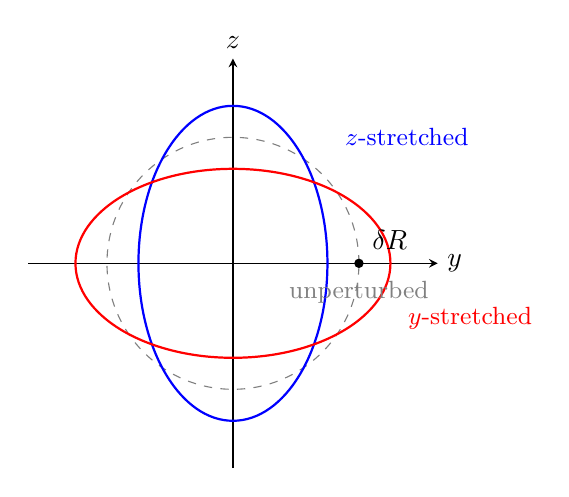
\begin{tikzpicture}[>=stealth, scale=1.0]
  \draw[->] (-2.6,0)--(2.6,0) node[right] {$y$};
  \draw[->] (0,-2.6)--(0,2.6) node[above] {$z$};
  \draw[gray, dashed] (0,0) circle (1.6);
  \draw[blue, thick] (0,0) ellipse (1.2 and 2.0);
  \draw[red,  thick] (0,0) ellipse (2.0 and 1.2);
  \node[circle,fill,inner sep=1.2pt,label=above right:{$\delta R$}] at (1.6,0) {};
  \node[blue, right] at (1.3,1.6) {\small $z$-stretched};
  \node[red,  right] at (2.1,-0.7) {\small $y$-stretched};
  \node[gray, below] at (1.6,-0.1) {\small unperturbed};
\end{tikzpicture}
\end{center}

\subsection*{(d) Total gravitational-wave luminosity}

Integrate $\mathcal F_r$ over the sphere $4\pi r^2$ to obtain the standard Einstein quadrupole luminosity in terms of the trace-free reduced mass-quadrupole $\bar Q_{ij}=Q_{ij}-\tfrac13 Q^k{}_k\delta_{ij}$ with $Q_{ij}\equiv I_{ij}/c^2$:
\begin{equation}
\mathcal L=\frac{G}{5c^5}\bigl\langle\dddot{\bar Q}_{ij}\dddot{\bar Q}^{ij}\bigr\rangle.
\label{eq:Lstd}
\end{equation}
Read off $Q_{zz}=\mu(L+a\cos\omega t)^2/2$ with all other $Q_{ij}=0$. Take the trace:
\[
Q^k{}_k=Q_{zz}.
\]
Form the trace-free components:
\[
\bar Q_{zz}=Q_{zz}-\tfrac13 Q_{zz}=\tfrac23 Q_{zz},\qquad \bar Q_{xx}=\bar Q_{yy}=-\tfrac13 Q_{zz}.
\]
Expand $Q_{zz}$ using $\cos^2\omega t=\tfrac12(1+\cos 2\omega t)$:
\[
Q_{zz}=\tfrac{\mu}{2}\bigl[L^2+2La\cos\omega t+a^2\cos^2\omega t\bigr].
\]
Apply the identity:
\[
Q_{zz}=\tfrac{\mu}{2}\Bigl[L^2+\tfrac{a^2}{2}+2La\cos\omega t+\tfrac{a^2}{2}\cos 2\omega t\Bigr].
\]
Differentiate three times in $t$ (constants drop; $\cos n\omega t\xrightarrow{(d/dt)^3} n^3\omega^3\sin n\omega t$):
\[
\dddot Q_{zz}=\tfrac{\mu}{2}\bigl[2La\omega^3\sin\omega t+\tfrac{a^2}{2}\cdot 8\omega^3\sin 2\omega t\bigr].
\]
Simplify the coefficients:
\[
\dddot Q_{zz}=\mu\bigl[La\omega^3\sin\omega t+2a^2\omega^3\sin 2\omega t\bigr]\equiv\mu S(t).
\]
Square the source:
\[
S^2=L^2a^2\omega^6\sin^2\omega t+4a^4\omega^6\sin^2 2\omega t+4La^3\omega^6\sin\omega t\sin 2\omega t.
\]
Apply $\langle\sin^2\omega t\rangle=\langle\sin^2 2\omega t\rangle=\tfrac12$ and the orthogonality of $\sin\omega t,\sin 2\omega t$:
\[
\langle S^2\rangle=\tfrac12 L^2a^2\omega^6+2a^4\omega^6.
\]
Factor $\tfrac12 a^2\omega^6$:
\[
\langle S^2\rangle=\tfrac12 a^2\omega^6\bigl(L^2+4a^2\bigr).
\]
Sum the trace-free squared components, using $\dddot{\bar Q}_{zz}=(2/3)\mu S$, $\dddot{\bar Q}_{xx}=\dddot{\bar Q}_{yy}=-(1/3)\mu S$:
\[
\dddot{\bar Q}_{ij}\dddot{\bar Q}^{ij}=\bigl(\tfrac{4}{9}+2\cdot\tfrac{1}{9}\bigr)\mu^2 S^2.
\]
Combine the fractions:
\[
\dddot{\bar Q}_{ij}\dddot{\bar Q}^{ij}=\tfrac{2}{3}\mu^2 S^2.
\]
Average:
\[
\langle\dddot{\bar Q}_{ij}\dddot{\bar Q}^{ij}\rangle=\tfrac{2}{3}\mu^2\cdot\tfrac12 a^2\omega^6(L^2+4a^2)=\tfrac{\mu^2 a^2\omega^6(L^2+4a^2)}{3}.
\]
Insert into \eqref{eq:Lstd}:
\[
\mathcal L=\frac{G}{5c^5}\cdot\frac{\mu^2 a^2\omega^6(L^2+4a^2)}{3}.
\]
Multiply the constants:
\begin{equation}
\boxed{\ \mathcal L=\frac{G\mu^2\omega^6 a^2\bigl(L^2+4a^2\bigr)}{15\,c^5}.\ }
\label{eq:Lboxed}
\end{equation}

\subsection*{(e) Energy radiated per period}

Multiply the luminosity by the period $T=2\pi/\omega$:
\[
\Delta E=\mathcal L\,T=\frac{G\mu^2\omega^6 a^2(L^2+4a^2)}{15c^5}\cdot\frac{2\pi}{\omega}.
\]
Simplify the $\omega$ power:
\[
\Delta E=\frac{2\pi G\mu^2\omega^5 a^2(L^2+4a^2)}{15c^5}.
\]
Compute the maximum speed of each mass from $\dot z_{1,2}=\pm\tfrac12 a\omega\sin\omega t$:
\[
v_{\max}=\frac{a\omega}{2}\ \Longrightarrow\ a^2\omega^2=4v_{\max}^2.
\]
Define a separation-scale velocity:
\[
v_L\equiv\frac{L\omega}{2}\ \Longrightarrow\ L^2\omega^2=4v_L^2.
\]
Rewrite $\omega^5 a^2$ using the first relation:
\[
\omega^5 a^2=\omega^3\cdot a^2\omega^2=4\omega^3 v_{\max}^2.
\]
Substitute:
\[
\Delta E=\frac{2\pi G\mu^2}{15c^5}\cdot 4\omega^3 v_{\max}^2\bigl(L^2+4a^2\bigr)=\frac{8\pi G\mu^2\omega^3 v_{\max}^2(L^2+4a^2)}{15c^5}.
\]
Replace $L^2=4v_L^2/\omega^2$ and $4a^2=16v_{\max}^2/\omega^2$:
\[
\Delta E=\frac{8\pi G\mu^2\omega^3 v_{\max}^2}{15c^5}\cdot\frac{4v_L^2+16v_{\max}^2}{\omega^2}.
\]
Collect the $\omega$ factors:
\[
\Delta E=\frac{8\pi G\mu^2\omega v_{\max}^2(4v_L^2+16v_{\max}^2)}{15c^5}.
\]
Factor a 4:
\begin{equation}
\boxed{\ \Delta E=\frac{32\pi G\mu^2\omega\,v_{\max}^2}{15c^5}\bigl(v_L^2+4v_{\max}^2\bigr).\ }
\label{eq:DeltaEbox}
\end{equation}

\textbf{Discussion of $L/a$.}
\begin{itemize}
\item $L/a\gg 1$ (small radial oscillation about a large separation): the $\omega$-harmonic dominates, $\Delta E\approx\frac{2\pi G\mu^2\omega^5 L^2 a^2}{15c^5}=\frac{32\pi G\mu^2\omega v_L^2 v_{\max}^2}{15c^5}$. Energy loss grows as $(L/a)^2$ at fixed $a$, so the radiation is sourced by the mass-monopole modulation about a large equilibrium length.
\item $L/a\to 0$ (pure breathing through the centre): only the $2\omega$ harmonic survives, $\Delta E\to\frac{8\pi G\mu^2\omega^5 a^4}{15c^5}=\frac{128\pi G\mu^2\omega v_{\max}^4}{15c^5}$. Independent of $L$; this is the lowest-order quadrupole emission of a symmetric oscillator.
\item Crossover at $L/a\sim 2$: the two contributions are comparable, and the GW signal contains a clean two-tone spectrum at $\omega$ and $2\omega$.
\end{itemize}

\end{document}
